\documentclass[9pt,twocolumn,twoside]{osajnl}
%% Please use 11pt if submitting to AOP
% \documentclass[11pt,twocolumn,twoside]{osajnl}
\journal{ol} % Choose journal (ao, aop, josaa, josab, ol, optica, pr)

% See template introduction for guidance on setting shortarticle option
\setboolean{shortarticle}{true}
% true = letter / tutorial
% false = research / review article
% (depending on journal).

\title{Generation of entangled states of light using discrete solitons in waveguide arrays}

\author[1,*]{V.O. Martynov}
\author[2]{V. O. Munyaev}
\author[1,2]{L. A. Smirnov}

\affil[1]{Institute of Applied Physics of the Russian Academy of Sciences, Nizhny Novgorod, 603950, Russia}
\affil[2]{Department of Control Theory, Nizhny Novgorod State University, Nizhny Novgorod, 603950, Russia}

\affil[*]{Corresponding author: martvo@ipfran.ru}

%% To be edited by editor
% \dates{Compiled \today}

%\ociscodes{(140.3490) Lasers, distributed feedback; (060.2420) Fibers, polarization-maintaining;(060.3735) Fiber Bragg gratings.}

%% To be edited by editor
% \doi{\url{http://dx.doi.org/10.1364/XX.XX.XXXXXX}}

\begin{abstract}
We study the quantum properties of light propagating through an array of coupled nonlinear waveguides and forming a discrete soliton in the classical limit. We demonstrate the possibility of using such quasi-solitons to form continuous variables entanglement between the particular pair of waveguides. We also show that there is a promising opportunity to entangle several pairs of waveguides independently. According to our analysis, the entanglement appears for the input laser field's arbitrary high intensity. Hence, it does not require a specific material with an extreme nonlinearity coefficient. Taking the weak absorption in the waveguide media into account results does not influence the discussed process too much.
\end{abstract}

\setboolean{displaycopyright}{true}
\usepackage{bm}
\begin{document}

\maketitle

On-chip integrated optical waveguide circuits open a wide variety of possibilities to manipulate quantum states of light~\cite{zoubi_quantum_2017, silverstone_-chip_2014, matthews_manipulation_2009, kruse_dual-path_2015}. 
One of the most promising usage of such devices is implementation of various quantum informatics algorithms~\cite{nielsen_quantum_2000}. Entangled states of light are the key element of quantum information processing. 
Development of integrated devices which generate such states using ordinary laser sources as their input appears to be an important problem. 
Recently, there have been proposed a number of schemes~\cite{belsley_generating_2020, guo_parametric_2017, caspani_integrated_2017, solntsev_path-entangled_2017, yang_manipulation_2014} to form entanglement between optical modes in different waveguides. 
These schemes are based on down-conversion processes in nonlinear media. 
They require the use of specific materials and waveguide geometry, which complicates the design of discussed devices. 
An alternative approach might be to use nonlinear self-action process which is more common and occurs in all materials with cubic nonlinearity. 
Currently, the possibility of using this process to generate entangled states is poorly studied. 
Here we propose to use an array of coupled waveguides with cubic nonlinearity to generate continuous variables entanglement~\cite{weedbrook_gaussian_2012}. 
Such objects are well studied from classical nonlinear dynamics point of view. 
It is known that there is a large variety of discrete solitons in such arrays~\cite{kevrekidis_discrete_2009, christodoulides_discretizing_2003}.
Taking quantum effects into account, the propagation of such field distributions can lead to nonclassical photon statistics. 
Such effect is known for continuous solitons~\cite{corney_quantum_2001, lai_entangled_2009}.
We will show that the similar behavior present in the discussed system.
The basic idea is that due to nonlinearity, the photon statistics will change as light travels through the waveguide.
\begin{figure}[h!]
	\centering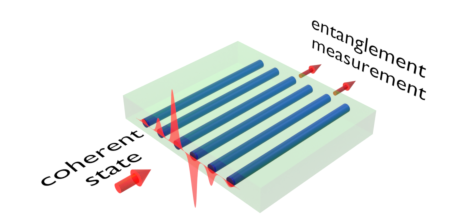
\includegraphics[width=7cm]{fig1}
	\caption{Schematic depiction of the quantum light propagation along an array of nonlinear waveguides.}
	\label{fig:schema}
\end{figure}
And the interaction between the optical modes of the waveguides will transform this non-classical state of light into an entangled one. 

\par
We consider an array consisting of $N$ single-mode waveguides~(Fig.~\ref{fig:schema}). 
A long laser pulse is sent to the input of each waveguide. Propagation of the pulse may be described in terms of slowly varying field operators $\hat{\psi}_{k}\left(x,t\right)$, where $k$ is the index of a waveguide, $x$ is the coordinate along array. The Hamiltonian of system consists of two parts:
\begin{equation}\label{eg:base_ham}
	\hat{H}=\hat{H}_s + \hat{H}_i.
\end{equation}
$\hat{H}_s$ refers to the independent propagation of light along individual waveguides.
In the slowly varying envelope and rotating-
wave approximations it equals~\cite{drummond_quantum_2014}: 
\begin{equation}
	\hat{H}_s = \sum^{N}_{k=1}\int dx\left[\dfrac{iv}{2}\left(\hat{\psi}^{\dag}_k\nabla\hat{\psi}^{\phantom{\dag}}_k - \nabla\hat{\psi}^{\dag}_n\hat{\psi}^{\phantom{\dag}}_k\right) +\dfrac{U}{2}\hat{\psi}^{\dag2}_k\hat{\psi}^{\phantom{\dag}2}_k\right], 
\end{equation}
v is group velocity. Hereinafter we assume that $\hbar=1$. $\hat{H}_i$ is the Hamiltonian which describes interaction of optical field in different waveguides. In case of weak coupling it equals~\cite{agarwal_quantum_2012}:
\begin{equation}
	\hat{H}_i = \sum^{N-1}_{k=1}\int \kappa\hat{\psi}^{\dag}_k\hat{\psi}^{\phantom{\dag}}_{k+1} dx +\rm{H.c.}
\end{equation}
Using Hamiltonian~\eqref{eg:base_ham} one can derive Heisenberg equations:
\begin{equation}
	\begin{array}{r}
		\left[-v\dfrac{\partial}{\partial x} + \dfrac{\partial}{\partial t}\right]\hat{\psi}^{\phantom{\dag}}_k\!\left(x,\!t\!\right) = -i\kappa\left[\hat{\psi}^{\phantom{\dag}}_{k-1}\!\left(x,\!t\!\right) + \hat{\psi}^{\phantom{\dag}}_{k+1}\!\left(x,\!t\!\right)\right] \\ -iU\hat{\psi}^{\dag}_k\!\left(x,\!t\!\right)\hat{\psi}^{\phantom{\dag}}_{k}\!\left(x,\!t\!\right)\hat{\psi}^{\phantom{\dag}}_{k}\!\left(x,\!t\!\right).
	\end{array}
\end{equation}
To simplify further calculations, we perform them in a moving frame using substitution $t_v = t - x/v$. Also we normalize distance $x \rightarrow z = \kappa x / v$:
\begin{equation}\label{eq:heis}
	\begin{array}{r}
		\dfrac{\partial}{\partial z}\hat{\psi}^{v}_k\!\left(z,\!t_v\!\right) = i\left[\hat{\psi}^{v}_{k-1}\!\left(z,\!t_v\!\right) + \hat{\psi}^{v}_{k+1}\!\left(z,\!t_v\!\right)\right] \\ +iL\hat{\psi}^{\dag v}_k\!\left(z,\!t_v\!\right)\hat{\psi}^{v}_{k}\!\left(z,\!t_v\!\right)\hat{\psi}^{v}_{k}\!\left(z,\!t_v\!\right),
	\end{array}
\end{equation}
where $L=Uv/\kappa$ and
\begin{equation}
	\hat{\psi}^{v}_k\!\left(z,\!t_v\!\right) = \hat{\psi}^{\phantom{\dag}}_k\!\left(\dfrac{vz}{\kappa},\!t - \dfrac{z}{\kappa}\!\right).
\end{equation}
$t_v$ in equations~\eqref{eq:heis} $t_v$ s just a parameter so in further calculations we omit it assuming that it is always the same and corresponds to the center of the input pulses. 
To calculate evolution of light field along the array based on equations~\eqref{eq:heis} we assume that quantum state of light is Gaussian for every value of $v$. 
This mean, that Sudarshan-Glauber P distribution has Gaussian profile. 
For such distributions cumulants~\cite{gardiner_stochastic_2009} $\ll\hat{X}_1\cdot\hat{X}_2\cdot\hat{X}_3\gg$ and $\ll\hat{X}_1\cdot\hat{X}_2\cdot\hat{X}_3\cdot\hat{X}_4\gg$ equal to zero if $\hat{X}_l$ takes a value from the set $\left\{\hat{\psi}^{v}_{k}, \hat{\psi}^{\dag v}_{k} \right\}$ in such a way that the products are normally ordered. This fact allows using the following relations:


\begin{equation}
	\begin{array}{r}
		\langle \hat{X}_1\!\cdot\!\hat{X}_2\!\cdot\!\hat{X}_3\rangle = \langle\hat{X}_1\rangle\langle\hat{X}_2\!\cdot\!\hat{X}_3\rangle + \langle\hat{X}_2\rangle\langle\hat{X}_1\!\cdot\!\hat{X}_3\rangle  \,\,\,\,\,\,\,\,\,\,\,\,\,\,\,\,\,\,\,\,\,\,\,\,\,\\+ \langle\hat{X}_3\rangle\langle\hat{X}_1\!\cdot\!\hat{X}_2\rangle - 2\langle\hat{X}_1\rangle \langle\hat{X}_2\rangle\langle\hat{X}_3\rangle \\
		\langle \hat{X}_1\!\cdot\!\hat{X}_2\!\cdot\!\hat{X}_3\!\cdot\!\hat{X}_4\rangle \!=\! \langle\hat{X}_1\!\cdot\!\hat{X}_2\rangle\langle\hat{X}_3\!\cdot\!\hat{X}_4\rangle \!+\!  \langle\hat{X}_1\!\cdot\!\hat{X}_3\rangle\langle\hat{X}_2\!\cdot\!\hat{X}_4\rangle \\+ \langle\hat{X}_1\!\cdot\!\hat{X}_4\rangle\langle\hat{X}_2\!\cdot\!\hat{X}_3\rangle - 2\langle\hat{X}_1\rangle \langle\hat{X}_2\rangle\langle\hat{X}_3\rangle\langle\hat{X}_4\rangle
	\end{array}
\end{equation}
to derive a closed set of equations for quantities $\alpha_k = \sqrt{L} \langle\hat{\psi}^{v}_{k}\rangle$, $\Delta^{a}_{k,l} = L \langle\hat{\psi}^{v}_{k}\hat{\psi}^{v}_{l}\rangle - \alpha^{\phantom{*}}_k\alpha^{\phantom{*}}_l$ and $\Delta^{n}_{k,l} = L \langle\hat{\psi}^{\dag v}_{k}\hat{\psi}^{v}_{l}\rangle - \alpha^{*}_k\alpha^{\phantom{*}}_l$~\cite{tikhonenkov_quantum_2007}: 
\begin{equation}\label{eq:second_order}
	\begin{array}{c}
		\dfrac{\partial}{\partial z}\alpha_{k}\! =\! i\left(\alpha_{k-1}\! +\! \alpha_{k+1} \right) \!+\! i\left|\alpha^{\phantom{*}}_{k}\!\right|^{2}\alpha^{\phantom{*}}_{k} \!\!+\! i\left(2\alpha^{\phantom{*}}_{k}\Delta^{n}_{k,k} \!+\! \alpha^{*}_{k}\Delta^{a}_{k,k}\right),\\
		\dfrac{\partial}{\partial z}\Delta^{n}_{k,l} = i\left(\Delta^{n}_{k,l+1} + \Delta^{n}_{k,l-1} - \Delta^{n}_{k+1,l} - \Delta^{n}_{k-1,l}\right) \\+ 2i\left(\Delta^{n}_{l,l} - \Delta^{n}_{k,k} + \left|\alpha^{\phantom{*}}_{l}\!\right|^{2} -\left|\alpha^{\phantom{*}}_{k}\right|^{2}\right)\Delta^{n}_{k,l}  \\
		+ i\left(\Delta^{a*}_{k,l}\Delta^{a}_{l,l} - \Delta^{a}_{k,l}\Delta^{a*}_{k,k} + \alpha^{2}_{l}\Delta^{a*}_{k,l} - \alpha^{*2}_{k}\Delta^{a}_{k.l}\right), \\
		\dfrac{\partial}{\partial z}\Delta^{a}_{k,l} = i\left(\Delta^{a}_{k,l+1} + \Delta^{a}_{k,l-1} + \Delta^{a}_{k+1,l} + \Delta^{a}_{k-1,l}\right)  \\+ 2i\left(\Delta^{n}_{k,k} + \Delta^{n}_{l,l} + \left|\alpha^{\phantom{*}}_{k}\right|^{2} + \left|\alpha^{\phantom{*}}_{l}\!\right|^{2}\right)\Delta^{a}_{k,l}  \\
		+ i\left(\Delta^{a}_{k,k} + \alpha^{2}_{k}\right)\Delta^{n}_{k,l} + i\left(\Delta^{a}_{l,l} + \alpha^{2}_{l}\right)\Delta^{n*}_{k,l} \\+ i\dfrac{L}{2}\delta_{k,l}\left(\alpha^{2}_{k} + \alpha^{2}_{l} + \Delta^{a}_{k,k} + \Delta^{a}_{l,l}\right).
	\end{array}
\end{equation}
\par
Before we start solving the equations~\eqref{eq:second_order}
we need to define boundary conditions at plane $z=0$. 
We assume that the quantum state of light is a multi mode coherent state at the input of the array. For such sort of states $\Delta^{a}_{k,l}$ and $\Delta^{n}_{k,l}$ equal zero for every $k,l = 1\ldots N$. So it is enough to specify the distribution of values $\alpha_k\!\left(z=0\right)$. Before we do so it should be noted that if in~\eqref{eq:second_order} one set $L=0$ the system of equations will be reduced to:
\begin{equation}\label{eq:classic}
	\dfrac{\partial}{\partial z}\alpha_{k}\! =\! i\left(\alpha_{k-1}\! +\! \alpha_{k+1} \right) \!+\! i\left|\alpha^{\phantom{*}}_{k}\!\right|^{2}\alpha^{\phantom{*}}_{k}.
\end{equation}
We want to emphasize here that $ L = 0 $ does not mean that we are neglecting nonlinearity. 
Instead, it means that the number of photons in optical modes tends to infinity, which can be interpreted as the transition to the classical physics limit. 
Equations~\eqref{eq:classic} have solutions which are called discrete solitons~\cite{kevrekidis_discrete_2009}.  
To find them let's look for solution having the form $\alpha_{k} = \beta_k e^{i\omega z}$. Here $\beta_k$ are real numbers that doesn't depend on $z$. 
For $\alpha_{k}$ to satisfy~\eqref{eq:classic} these numbers should obey next equations:
\begin{equation}\label{eq:alg}
	-\omega \beta_k +\beta_{k+1 } + \beta_{k+1} + \beta^{3}_k = 0.
\end{equation}
For equations~\eqref{eq:alg} there is a number of solutions sets parameterized by parameter $\omega$  and which exist only when $\omega > 2$.
Some of these sets are linearly stable if $\omega$ is large enough and we will use them as boundary condition for~\eqref{eq:second_order}.  
On the top row of Fig.~\ref{fig:structure} some examples of such solutions are depicted.  
It should be noted that the equations~\eqref{eq:classic} can be considered a discrete analogue of the nonlinear Schrödinger equation~(NLSE). 
For this equation there is a well-known soliton solution quantum properties of which have been studied in several papers~\cite{corney_quantum_2001,lai_entangled_2009}. 
Discrete analog of such solution is shown on Fig.~\ref{fig:structure}(a). 
In case of infinite number of waveguides and $\omega\rightarrow 2$ mentioned discrete soliton should become similar to NLSE-soliton and have the same quantum properties. 
In the further discussion, we will focus on situations where discrete effects are significant. 
This means that we will use discrete solitons corresponding to large values of $\omega$ and having no continuous analogs, as shown in Fig.~\ref{fig:structure}(b) and Fig.~\ref{fig:structure}(c).
\par
\begin{figure*}[h!]
	\centering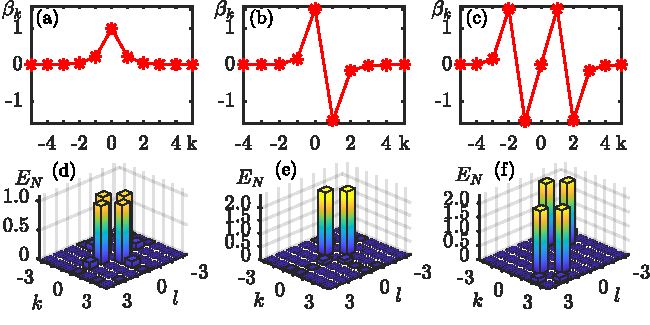
\includegraphics{fig2}
	\caption{Top row represents the structure of discrete soliton solutions for light propagation in an array of waveguides with cubic nonlinearity. The bottom row shows the distributions of bipartite entanglement between different pairs of waveguides for the corresponding discrete soliton from the top row. The logarithmic negativity~($E_N$) is used to quantitatively describe entanglement. (a) and (d) are based on calculations for $\omega = 5.0$, for the other sub-figures $\omega = 10.0$. To calculate distributions in the bottom row $L=0.01$ is used.}
	\label{fig:structure}
\end{figure*}
By solving equations~\eqref{eq:second_order} we want to study the quantum properties of the light field.
First of all we are interested in the entanglement that forms between the modes of different optical waveguides.
We will limit our consideration only by studying bipartite entanglement~\cite{gebremariam_tesfahannes_generation_2020, tura_detecting_2014}.
For this purpose we will use quantity called logarithmic negativity~($E_N$)~\cite{vidal_computable_2002} and will calculate it for different pairs of waveguides. 
In case of Gaussian quantum states $E_N$ for two waveguides with indexes $k$ and $l$ can be calculated based on correlation matrix $\bm{\sigma}$:
\begin{equation}\label{eq:cov_matr}
	\sigma_{m,n}=\langle\hat{\xi}_{m}\hat{\xi}_{n}+\hat{\xi}_{m}\hat{\xi}_{n}\rangle\bigl/2\bigr.-\langle\hat{\xi}_{m}\rangle\langle\hat{\xi}_{n}\rangle,    
\end{equation}
where indexes $m$ and $n$ take value from $1$ to $4$, and $\hat{\xi}_{m}$ and $\hat{\xi}_{n}$ are the corresponding components of a four-dimensional vector $\hat{\bm{\xi}}=\left(\,\hat{q}_{k},\hat{p}_{k},\,\hat{q}_{l},\,\hat{p}_{l}\,\right)^{T}$:
\begin{equation}\label{eq:qp}
	\hat{q}_{k,l}=\frac{1}{\sqrt{2}}\left(\hat{\psi}^{\dag v}_{k,l}+\hat{\psi}^{v}_{k,l}\right),\hspace{2.5mm}\hat{p}_{k,l}=\frac{i}{\sqrt{2}}\left(\hat{\psi}^{\dag v}_{k,l}-\hat{\psi}^{v}_{k,l}\right).
\end{equation}
using matrix~\eqref{eq:cov_matr} it is possible to calculate logarithmic negativity:
\begin{equation}\label{eq:EN}
	E_N = -\dfrac{1}{2}\sum_r \rm{log}_2 \rm{min}\left\{1, 2\left|l_r\right|\right\},
\end{equation}
where $l_r$ are symplectic eigenvalues of matrix $\bm{\sigma}$.
\par
Before we discuss the results of calculations for quantum entanglement we should do a remark about Gaussian approximation we are using. 
The problem is that equations~\eqref{eq:heis} do not preserve the property of a quantum state to be Gaussian. 
But the initial quantum state is Gaussian. 
So we may assume that our approximation is valid for a certain distance of pulse propagation. 
And we need to estimate this distance to make sure the results we get are correct.
To solve this problem we consider the next order of cumulants expansion. 
We let $\ll\hat{X}_1\cdot\hat{X}_2\cdot\hat{X}_3\gg$ to be non zero but higher order cumulants still remains zero.
In this assumption we can derive the set of equations to calculate third order cumulant and compare it with zero.
We calculate next quantity:
\begin{equation}
Err \!= \!\!\dfrac{\max\!\left\{\underset{k,l}{\max}\!\left|\ll\!\hat{\psi}^{\dag v}_{k}\!\cdot\!\hat{\psi}^{ v}_{k}\!\cdot\!\hat{\psi}^{ v}_{l}\!\!\gg\right|\!,\underset{k,l}{\max}\!\left|\ll\!\hat{\psi}^{ v}_{k}\!\cdot\!\hat{\psi}^{ v}_{k}\!\cdot\!\hat{\psi}^{ v}_{l}\!\!\gg\right|\right\}}
{\max\left\{\underset{k,l}{\max}\left|\langle\hat{\psi}^{\dag v}_{k}\!\cdot\!\hat{\psi}^{ v}_{k}\!\cdot\!\hat{\psi}^{ v}_{l}\rangle\right|,\underset{k,l}{\max}\left|\langle\hat{\psi}^{ v}_{k}\!\cdot\!\hat{\psi}^{ v}_{k}\!\cdot\!\hat{\psi}^{ v}_{l}\rangle\right|\right\}}\!.
\end{equation}
Here we divide the maximum value between all cumulants we need to derive equations~\eqref{eq:second_order} by maximum value of averages which we calculate using the fact that corresponding cumulant is zero.
Thus, the Gaussian approximation is valid when the value of $Err$ is much less than one.
Dependency of $Err$ on the distance of light propagation along the array is shown on Fig.~\ref{fig:results}(a) by red dotted line. It is calculated for discrete soliton having filed distribution like the one shown on Fig.~\ref{fig:structure}(b) and parameters: $\omega = 10$, $L=0.01$.
From the curve one may notice that the defined quantity grows very slow for $z<1$, but after that point it increases dramatically.
This means that our approximation is valid until propagation distance is less than one.
This threshold distance depends weakly on the discrete soliton type and parameters of the system $\omega$ and $L$. 
All further calculations will be limited by this distance.
\par
\begin{figure}[h!]
	\centering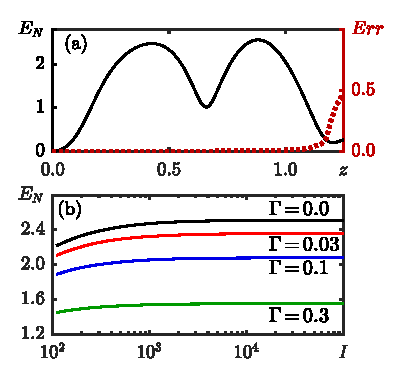
\includegraphics[width=7cm]{fig3}
	\caption{(a) Evolution of quantum properties of light propagating along an array of nonlinear waveguides. 
		The black solid line corresponds to the evolution of logarithmic negativity, the red dotted line is the evolution of the parameter that determines the applicability of the Gaussian approximation. (b) Dependence of the maximum value of $E_N$ attained during the propagation of light along the array on the light intensity in the central waveguide. All curves are calculated for a soliton of~Fig.\ref{fig:structure}(b) and $\omega=10.0$, (a) is calculated using $L=0.01$.} 
	\label{fig:results}
\end{figure}
Our calculations show that the distribution of the average photons number between waveguides does not change on propagation distance for which Gaussian approximation is valid. 
It remains the same as it is on the input of an array. 
At the same time the discussed distance is enough for the quantum state to change enough to form entangled states.
An example of the evolution of logarithmic negativity~($E_N$) is shown in Fig.~\ref{fig:results}(a) with a black solid line.
It is calculated for two central waveguides of a discrete soliton with an amplitude distribution as in Fig.~\ref{fig:structure}(b), and the parameters are $\omega=10.0$ and $L=0.01$.
The discussed curve shows that $ E_N $ reaches its maximum value rather quickly. The maxima point is characterized by the greatest degree of entanglement that can be achieved in the system. 
For a given propagation distance, we will discuss further results.
Distributions of $E_N$ calculated for different pairs of waveguides and three types of discrete solitons are shown on Fig.~\ref{fig:structure} on the bottom line.
These images show that entanglement is formed mainly between central waveguides having maximal intensity.
For discrete analog of NLSE-soliton~(Fig.~\ref{fig:structure}(a,d)) bipartite entanglement is present only between the central waveguide and its nearest neighbors.
Moreover, as $\omega$ increases, the distribution of the average number of photons degenerates to a situation where almost all photons are in one waveguide. 
Of course, in such a situation, there is no entanglement in the system.
For the case of sign changing discrete solitons like depicted on Fig.~\ref{fig:structure}(b,c) bipartite entanglement present only for the pair of optical modes having maximal average photon number~(see Fig.~\ref{fig:structure}(e,f)). 
In our opinion, solitons of this kind are the most interesting from a practical point of view.
Our calculations show that when the complex amplitude of a soliton changes sign several times~(as in Fig.~\ref{fig:structure}(c)), entanglement is formed only between distinct pairs of waveguides.
In practice this fact can be used to construct optical integrated circuit generating multiple entangled states in parallel.
\par
For most optical materials, the cubic nonlinearity coefficient is relatively small. 
So, to form a discrete soliton, it is necessary to use laser pulses with a large number of photons.
It is important to understand what happens to the discussed entangled states when the intensity of the incoming light increases and we move to the limit that is usually considered classical.
To achieve this goal we should perform calculations for $L$ tending to zero.
The result is shown in Fig.~\ref{fig:results}(b) by black line. 
An interesting fact here is that the quantum state remains entangled as the intensity of the incoming light increases.
This result can be easily explained.
If we look at equations~\eqref{eq:second_order} we can notice that  variables $\Delta^{n}_{k,l}$ and $\Delta^{a}_{k,l}$ are small for small values of $L$.
We can linearize them and get a system of inhomogeneous equations.
It is clear that solution is proportional to source term $\Delta^{n,a}_{k,l}\sim L \cdot \alpha^2_k$. 
At the same time, the correlation matrix~\eqref{eq:cov_matr} which determines entanglement, is proportional to $\bm{\sigma}\sim \Delta^{n,a}_{k,l}/L$.
In combination these two facts lead to that $\bm{\sigma}$ does not depend on $L$. 
From the point of view of quasiprobability distributions, this means that the evolution of quadratures does not depend on the position of the distribution center.
\par
The last thing we want to mention here is the influence of absorption on the process of entangled states formations.
To consider absorption, we use a standard model of interaction with   a reservoir of an infinite number of harmonic oscillators~\cite{drummond_quantum_2014}.
This will result in additional terms in ~\eqref{eq:second_order} which have the form $-\Gamma \alpha_k / 2$, $-\Gamma \Delta^{n}_{k,l}$ and $-\Gamma \Delta^{a}_{k,l}$ for corresponding equations sets. 
Here $\Gamma$ is the absorption coefficient.
In the presence of absorption, the evolution of entanglement remains qualitatively the same.
The only thing that changes is the maximum value of logarithmic negativity that can be achieved in the system.
On Fig.~\ref{fig:results}(b) dependency of this quantity on intensity of input beams is shown for several values of $\Gamma$.
The entangled states of light are still formed even for relatively high absorption coefficients. 
In real experiment setups coupling coefficient $\kappa/v$ can be about  $1 \rm{cm}^{-1}$~\cite{solntsev_generation_2014}.
For such value $\Gamma=0.3$ corresponds to absorption $0.3 \rm{cm}^{-1}$ which is very high for typical optical materials.
\par
In conclusion we underline the achieved results.
We have studied the quantum properties of discrete solitons propagating through an array of cubic nonlinear waveguides.
Certain types of such field distributions form entangled states of light between optical modes of multiple pairs of coupled waveguides.
We propose that they can be used to create integrated optical devices for generating continuous-variable entangled states.
The advantage of such scheme is that discussed quasi-solitons are stable and do not require high quality of light field amplitude matching on the input of the array.
Also we have shown that entangled states are formed even in the case of using input sources with high intensities.
This means that proposed scheme does not require any specific materials with extremely high nonlinear coefficients.
Absorption which is present in all real materials also does not influence the entangled states generation process too much. 
There is an open question of the influence of the other sources of noise on the discussed process, such as Raman scattering or fluctuations of coupling coefficient.
However, this is the topic for future studies.
\section*{Acknowledgments}
The reported study was funded by RFBR according to the research project № 19-32-80038
\section*{Disclosures}
The authors declare no conflicts of interest.
%\section{Introduction}
%This legacy template is designed to assist with creating an article to submit to \emph{Applied Optics}, \emph{Advances in Optics and Photonics}, JOSA A, JOSA B, \emph{Optics Letters} or \emph{Optica}. See the OSA's \href{http://www.opticsinfobase.org/submit/style/}{Style Guide} and \href{http://www.opticsinfobase.org/submit/templates/}{Manuscript Templates} pages for more details. Please select the appropriate journal abbreviation (ao, aop, josaa, josab, ol, optica) in the document preamble.
%
%Use the shortarticle/false option for \emph{Applied Optics}, JOSA A, and JOSA B. Use the shortarticle/true option for \emph{Optics Letters}. For \emph{Advances in Optics and Photonics}, use the shortarticle/false option for Review Articles, and the shortarticle/true option for Tutorials.
%
%If you have a question while using this template on {Overleaf}, please use the help menu (``?'') on the top bar to search for help or ask us a question using our \href{https://www.overleaf.com/contact}{contact form}.
%
%\section{Examples of Article Components}
%\label{sec:examples}
%
%The sections below show examples of different article components.
%
%\section{Figures and Tables}
%
%It is not necessary to place figures and tables at the back of the manuscript. Figures and tables should be sized as they are to appear in the final article. Do not include a separate list of figure captions and table titles.
%
%Figures and Tables should be labelled and referenced in the standard way using the \verb|\label{}| and \verb|\ref{}| commands.
%
%\subsection{Sample Figure}
%
%Figure \ref{fig:false-color} shows an example figure.
%
%\begin{figure}[htbp]
%\centering
%\fbox{\includegraphics[width=\linewidth]{sample}}
%\caption{False-color image, where each pixel is assigned to one of seven reference spectra.}
%\label{fig:false-color}
%\end{figure}
%
%\subsection{Sample Table}
%
%Table \ref{tab:shape-functions} shows an example table.
%
%\begin{table}[htbp]
%\centering
%\caption{\bf Shape Functions for Quadratic Line Elements}
%\begin{tabular}{ccc}
%\hline
%local node & $\{N\}_m$ & $\{\Phi_i\}_m$ $(i=x,y,z)$ \\
%\hline
%$m = 1$ & $L_1(2L_1-1)$ & $\Phi_{i1}$ \\
%$m = 2$ & $L_2(2L_2-1)$ & $\Phi_{i2}$ \\
%$m = 3$ & $L_3=4L_1L_2$ & $\Phi_{i3}$ \\
%\hline
%\end{tabular}
%  \label{tab:shape-functions}
%\end{table}
%
%\section{Sample Equation}
%
%Let $X_1, X_2, \ldots, X_n$ be a sequence of independent and identically distributed random variables with $\text{E}[X_i] = \mu$ and $\text{Var}[X_i] = \sigma^2 < \infty$, and let
%\begin{equation}
%S_n = \frac{X_1 + X_2 + \cdots + X_n}{n}
%      = \frac{1}{n}\sum_{i}^{n} X_i
%\label{eq:refname1}
%\end{equation}
%denote their mean. Then as $n$ approaches infinity, the random variables $\sqrt{n}(S_n - \mu)$ converge in distribution to a normal $\mathcal{N}(0, \sigma^2)$.
%
%\section{Sample Algorithm}
%
%Algorithms can be included using the commands as shown in algorithm \ref{alg:euclid}.
%
%\begin{algorithm}
%\caption{Euclid’s algorithm}\label{alg:euclid}
%\begin{algorithmic}[1]
%\Procedure{Euclid}{$a,b$}\Comment{The g.c.d. of a and b}
%\State $r\gets a\bmod b$
%\While{$r\not=0$}\Comment{We have the answer if r is 0}
%\State $a\gets b$
%\State $b\gets r$
%\State $r\gets a\bmod b$
%\EndWhile\label{euclidendwhile}
%\State \textbf{return} $b$\Comment{The gcd is b}
%\EndProcedure
%\end{algorithmic}
%\end{algorithm}
%
%\subsection{Supplementary materials in OSA journals}
%OSA journals allow authors to include supplementary materials as integral parts of a manuscript. Such materials are subject to peer-review procedures along with the rest of the paper and should be uploaded and described using OSA's Prism manuscript system. Please refer to the \href{https://www.opticsinfobase.org/submit/style/supplementary_materials.cfm}{Author Guidelines for Supplementary Materials in OSA Journals} for more detailed instructions on labeling supplementary materials and your manuscript. Visualizations, Data Files, Datasets, and Code must be associated with a figure, table, or equation, OR be referenced in the results section of the manuscript. 
%
%\textbf{Authors may also include Supplemental Documents} (PDF documents with expanded descriptions or methods) with the primary manuscript. At this time, supplemental PDF files are not accepted for partner titles, JOCN and Photonics Research. To reference the supplementary document, the statement ``See Supplement 1 for supporting content.'' should appear at the bottom of the manuscript (above the References heading). Please note that to create text color for supplementary materials links, use of the command \\
%\verb|\textcolor{urlblue}{Visualization 1}| is preferred to using the command\\
%\verb|\url{Visualization 1}|.
%
%\begin{figure}[ht!]
%\centering\includegraphics{sample}
%\caption{(a) Three traps create three rings of magnetic nanoparticles. (b) The rings interact with one another.}
%\end{figure}
%
%
%\subsection{Sample Dataset Citation}
%
%1. M. Partridge, "Spectra evolution during coating," figshare (2014) [retrieved 13 May 2015], http://dx.doi.org/10.6084/m9.figshare.1004612.
%
%\subsection{Sample Code Citation}
%
%2. C. Rivers, "Epipy: Python tools for epidemiology" (Figshare, 2014) [retrieved 13 May 2015], http://dx.doi.org/10.6084/m9.figshare.1005064.
%
%\section{Funding}
%Content in the funding section will be generated entirely from details submitted to Prism. Authors may add placeholder text in the manuscript to assess length, but any text added to this section in the manuscript will be replaced during production and will display official funder names along with any grant numbers provided. If additional details about a funder are required, they may be added to the Acknowledgments, even if this duplicates information in the funding section. See the example below in Acknowledgements.
%
%\section{Acknowledgments}
%Acknowledgments should be included at the end of the document. The section title should not follow the numbering scheme of the body of the paper. Additional information crediting individuals who contributed to the work being reported, clarifying who received funding from a particular source, or other information that does not fit the criteria for the funding block may also be included; for example, ``K. Flockhart thanks the National Science Foundation for help identifying collaborators for this work.''
%
%\section{Disclosures}
%
%Disclosures should be listed in a separate section at the end of the manuscript. List the Disclosures codes identified on OSA's \href{http://www.osapublishing.org/submit/review/conflicts-interest-policy.cfm}{Conflict of Interest policy page}. If there are no disclosures, then list ``The authors declare no conflicts of interest.''
%
%Here are examples of disclosures:
%
%\medskip
%
%\noindent\textbf{Disclosures.} ABC: 123 Corporation (I,E,P), DEF: 456 Corporation (R,S). GHI: 789 Corporation (C).
%
%\medskip
%
%\noindent\textbf{Disclosures.} The authors declare no conflicts of interest.
%
%\section{References}
%
%Note that \emph{Optics Letters} and \emph{Optica} short articles use an abbreviated reference style. Citations to journal articles should omit the article title and final page number; this abbreviated reference style is produced automatically when the \emph{Optics Letters} journal option is selected in the template, if you are using a .bib file for your references.
%
%However, full references (to aid the editor and reviewers) must be included as well on a fifth informational page that will not count against page length; again this will be produced automatically if you are using a .bib file.
%
%\bigskip
%\noindent Add citations manually or use BibTeX. See %\cite{Zhang:14,OSA,FORSTER2007,testthesis,manga_rao_single_2007}.

% Bibliography
\bibliography{main}

% Full bibliography added automatically for Optics Letters submissions; the following line will simply be ignored if submitting to other journals.
% Note that this extra page will not count against page length
\bibliographyfullrefs{main}

%Manual citation list
%\begin{thebibliography}{1}
%\bibitem{Zhang:14}
%Y.~Zhang, S.~Qiao, L.~Sun, Q.~W. Shi, W.~Huang, %L.~Li, and Z.~Yang,
 % \enquote{Photoinduced active terahertz metamaterials with nanostructured
  %vanadium dioxide film deposited by sol-gel method,} Opt. Express \textbf{22},
  %11070--11078 (2014).
%\end{thebibliography}

\end{document}
